%---------------------------------------------------------------------------------------%	SECTION 4.1

%---------------------------------------------------------------------------------------

\section{The Riemann Integral.}

\begin{definition}
    Let $a,b \in \R$, with  $a<b$. We define a  \textbf{partition} of $[a,b]$ to be a set of points $P=\{x_0,x_1, \dots, x_n\}$ such that $a=x_0<x_1< \dots <x_n=b$.
    We define the \textbf{norm} of a partion $P=\{x_0,x_1, \dots, x_n\}$ to be the number:
    \begin{equation}
        ||P||=\max|x_j-x_{j-1}|
    \end{equation} 
    We call a \textbf{refiment} of a partition $P=\{x_0,x_1, \dots, x_n\}$ to be a partition $Q$ of  $[a,b]$ such that  $P \subseteq P$, and we say that $Q$ is  \textbf{finer} than $P$.
\end{definition}

\begin{figure}	
    \centering
    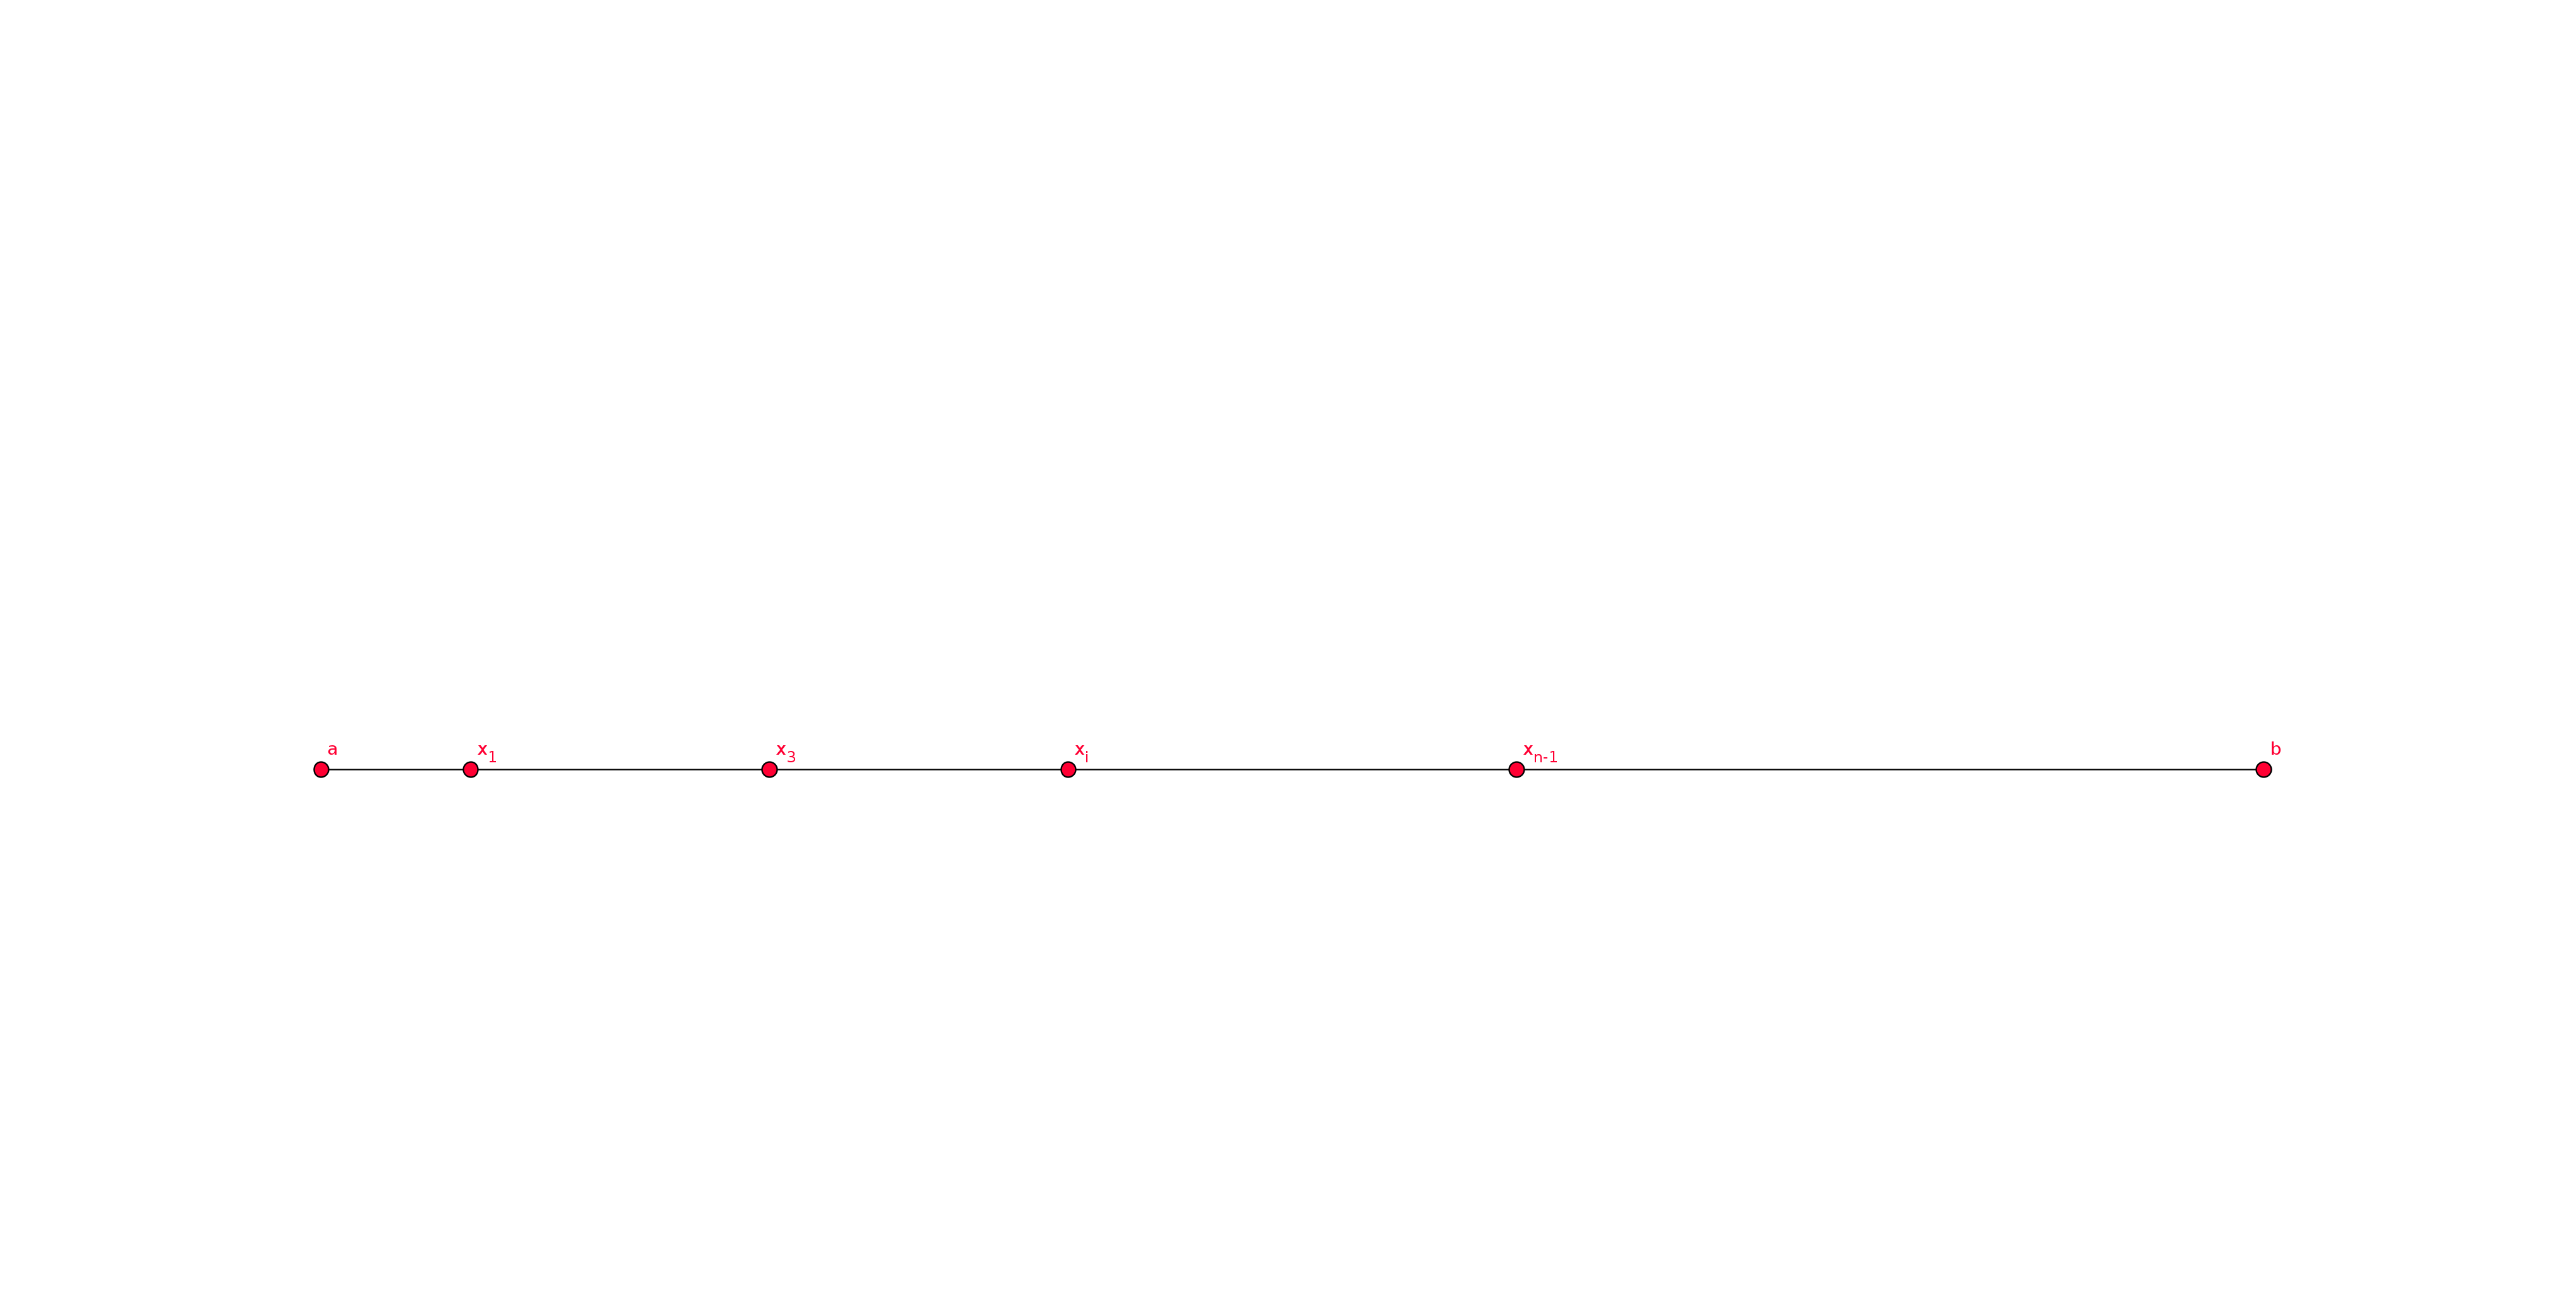
\includegraphics[scale = 0.3]{figures/partitionOfAnInterval.png}
    \caption{A Partition of the interval $[a,b]$.}
    \label{fig_5.1}
\end{figure}

\begin{example}[Dyadic Partitions]
    Let $P_n=\{\frac{j}{2^n}: j=0,1, \dots 2^n\}$, then $P_n$ is a partiton of  $[0,1]$, and  $P_m$ is finer than  $P_n$ if  $m>n$.
    Dyadic are good choices for partitions.
\end{example} 

If we have two partitions $P$ and  $Q$, in general, they may have no relation. But, $P \cup Q$ is a refinment of both  $P$ and  $Q$. Now if  $Q$ is finer than $P$, we see that  $||Q|| \leq ||P||$, that is the norm is a monotonically decreasing function of  $x_j$.

\begin{figure}
    \centering
    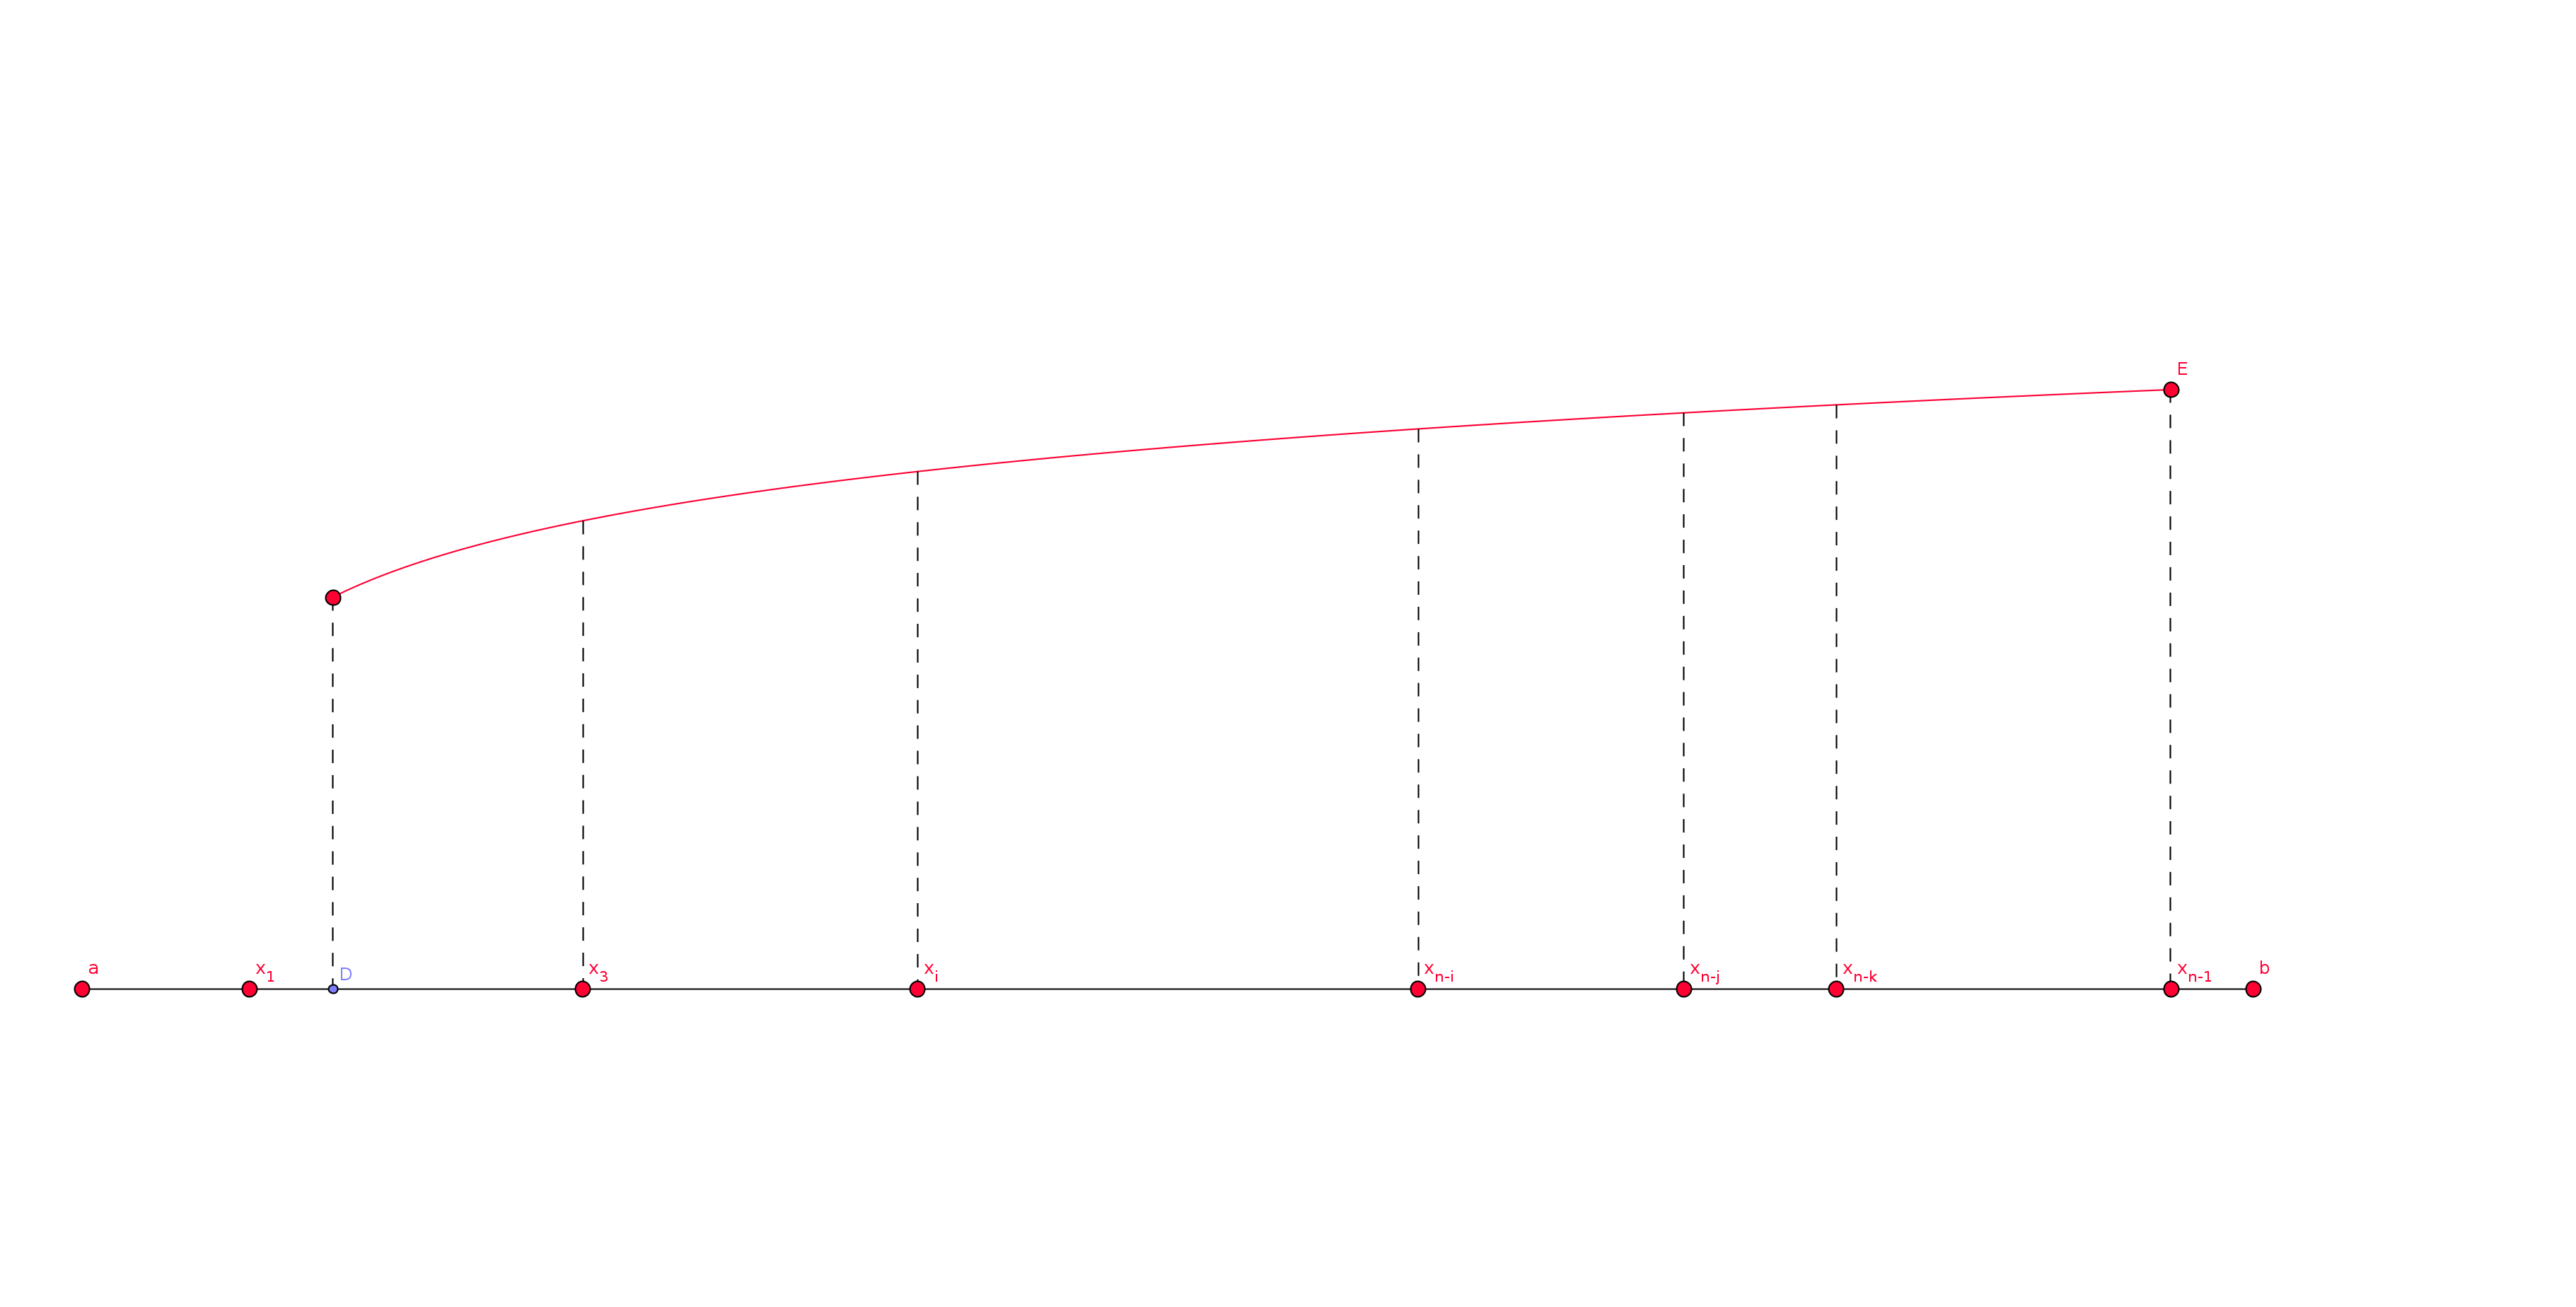
\includegraphics[scale = 0.5]{figures/partitionOfACurve.png}
    \caption{The Riemann Sum of a nonnegative bounded curve over the interval $[a,b]$.}
    \label{fig_5.2}
\end{figure}

\begin{definition}
    Let $a,b \in \R$ with  $a<b$ let $P=\{x_0,x_1, \dots, x_n\}$ be a partition of  $[a,b]$, and suppose that  $f:[a,b] \rightarrow \R$ is bounded. 
    We define the  \textbf{upper Riemann sum} of $f$ over  $P$ to be:
     \begin{equation}
         U(f,P)=\sum_{j=1}^{n}{M_j(f)(x_j-x_{j-1})}		
    \end{equation} 
    where $M_j(f)=\sup{f(x)}$ where  $x \in [x_{j-1},x_j]$.

We define the \textbf{lower Riemann sum} of $f$ over  $P$ to be:
     \begin{equation}
         L(f,P)=\sum_{j=1}^{n}{m_j(f)(x_j-x_{j-1})}
    \end{equation}
    Where $m_j(f)=\inf{f(x)}$ with  $x \in [x_{j-1},x_j]$
\end{definition}

\begin{remark}
    SUppose that $f(x)=\alpha$ is a constant function on  $[a,b]$. Then  $M_j(f)=m_j(f)=\alpha$, hence we see that
        \begin{equation*}
            U(f,P)=L(f,P)=\alpha\sum_{j=1}^{n}{x_j-x_{j-1}}=\alpha(b-a)
        \end{equation*} 
\end{remark}

\begin{remark}
    We have that $L(f,P) \leq U(f,P)$ for all  partitions $P$ and bounded functions  $f$, since $\inf{f} \leq \sup{f}$, so the relevant equalities follow.
\end{remark}

\begin{lemma}\label{5.1.1}
    If $P$ is any partition of  $[a,b]$, and there is a refinment of $P$, $Q$, then $L(f,P) \leq L(f,Q) \leq U(f,Q) \leq U(f,P)$. 
\end{lemma}
\begin{proof}
    Assume that $Q=P \cup \{x'\}$, with $x_{j-1}<x'<x_j$.
    Then $L(f,P)=\sum{m_j(f)(x_j-x_{j-a})}+m_j(f)(x_j-x'+x'-x_{j-1}) \leq \sum{m_j(f)(x_j-x_{j-1})}+m_{j_0'}(f)(x_{j_0}-x')+m_{j_0''}(f)(x'-x_j_0)=L(f,Q)$. We see that $inf{f}$ is increasing while $\sup{f}$ is decreasing, hence we get that  $U(f,Q) \leq U(f,P)$ by similar reasoning, and clearly  $L(f,Q) \leq U(f,Q)$.
\end{proof}
\begin{remark}
    What lemma \ref{5.1.1} says is that the lower sum is monotonically increasing while the upper sum is monotonically decreasing with respect to the refinment.
\end{remark}
